\documentclass[a4paper,14pt]{article}

\usepackage[12pt]{extsizes}
\usepackage{cmap}					% поиск в PDF
\usepackage{mathtext} 				% русские буквы в формулах
\usepackage[T2A]{fontenc}			% кодировка
\usepackage[utf8]{inputenc}			% кодировка исходного текста
\usepackage[english,russian]{babel}	% локализация и переносы
\usepackage{graphicx}
\usepackage{geometry}
\usepackage{amsmath}
\usepackage{amssymb}
\usepackage[table]{xcolor}
\setlength\extrarowheight{2pt}


\geometry{verbose, a4paper, tmargin=2cm, bmargin=2cm, lmargin=2cm, rmargin=2cm}
\author{Vysotsky Maxim}
\title{Отчёт}
\date{2025}

\begin{document}
	\begin{titlepage}
		\begin{center}
			{Министерство науки и высшего образования Российской Федерации
				НОВОСИБИРСКИЙ НАЦИОНАЛЬНЫЙ ИССЛЕДОВАТЕЛЬСКИЙ
				ГОСУДАРСТВЕННЫЙ УНИВЕРСИТЕТ (НГУ)}
		\end{center}
		\begin{center}
			{Физический факультет}
		\end{center}
		\begin{center}
			{Кафедра общей физики}
		\end{center}
		
		
		\vspace{7cm}
		{
			\begin{center}
				{\bf Лабораторная работа №1.1}\\
			Броуновское движение частиц в жидкости.
			\end{center}
		}
		\vspace{2cm}
		\begin{flushright}
			{Руководитель:\\ Ассистент\\
				Художитков В. Э.\\
                Старший преподаватель \\
                Кравцова А. Ю.\\
				Работу выполнил:\\
				Высоцкий М. Ю.\\
				\vspace{0.2cm}
				гр. 24301}
		\end{flushright}
		\vspace{3cm}
		\begin{center}
			Новосибирск, 2025
		\end{center}
	\end{titlepage}

\section{Теоретическое введение}
\hspace{\parindent}\textbf{Цель:} Изучить, какими законами можно описывать броуновское
движение, и каков физический смысл основных параметров этого движения. Поиск коэффициента перевода изображения из пикселей в мкм, поиск коэффициента диффузии жидкости.

\textbf{Оборудование}: микроскоп ОМ-П, веб-камера вмонтированная в микроскоп, объект-микрометр. 

\textbf{Броуновское движение} – это беспорядочное тепловое движение малых частиц,
взвешенных в жидкости или газе. 

Причинами броуновского движения в общем случае является хаотическое тепловое движение молекул среды, обуславливающее флуктуации импульса, передаваемого частицам в каждый момент времени. В жидкости связи между молекулами среды больше тепловых.

\begin{figure}[h]
    \centering
    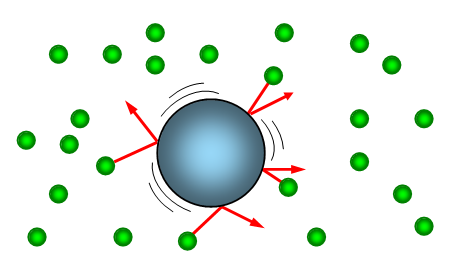
\includegraphics[scale=1]{brown.png}
    \caption{Броуновское движение.}
\end{figure}

И так как мы переходим на микроуровень (порядка 1 мкм), мы не можем руководствоваться законами Ньютона. Движение частиц имеет сугубо случайных характер. Когда хаотические тепловые флуктуации импульса, передаваемого
частице со стороны жидкости, превысят изменения импульса, определяемые изменением
потенциальной энергии шарика в поле тяготения за те же времена, тогда дальнейшим
движением частицы будут управлять уже эти тепловые флуктуации среды.

В силу вида траектории броуновской частицы (ломаная линия), мы не можем говорить о классическом определении скорости и ускорения этой самой частицы, и потому к ней неприменимы классические дифференциальные уравнения механики. Мы банально не можем взять производные в местах изгиба - левая и правая производные не будут равны. И потому законы, описывающие движение броуновской частицы, будут носить вероятностный характер.

\begin{figure}[h]
    \centering
    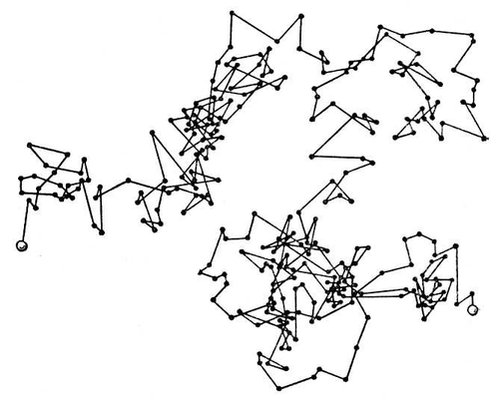
\includegraphics[scale=0.6]{brown1.jpg}
    \caption{Броуновское движение.}
\end{figure}

Поскольку флуктуации жидкости носят случайный
характер, то нас должно интересовать не конкретное поведение частицы в каждой точке
траектории, а некоторые средние характеристики ее движения. 

\textbf{Cтатистический ансамбль} – это совокупность сколь угодно большого числа одинаковых
физических систем («копий» данной системы), находящихся в одинаковых
макроскопических состояниях; при этом микроскопические состояния систем могут
принимать все возможные значения, совместимые с заданными значениями макроскопиче-
ских параметров, определяющих её макроскопическое состояние.

Cредний квадрат проекции смещения частицы вдоль OX:
$$
\overline{x^2} = 2Dt = 2Dn\tau
$$

Коэффициент диффузии D:
$$
D = \frac{kT}{6\pi\eta a}
$$

Сам коэффициент D является еще одним макропараметром системы частица-капля, который, также как и другие макропараметры, например. Р и Т, является статистическим средним микропроцессов, происходящих в данной системе.

\clearpage

\subsection{Ход работы}
\hspace{\parindent} Во-первых, построим движение броуновской частицы в осях XY. В силу сложной презентабельности, данные будут приложены отдельным файлом .xlsx, а фотографии в отдельной папке. 

\begin{figure}[ht!]
    \centering
    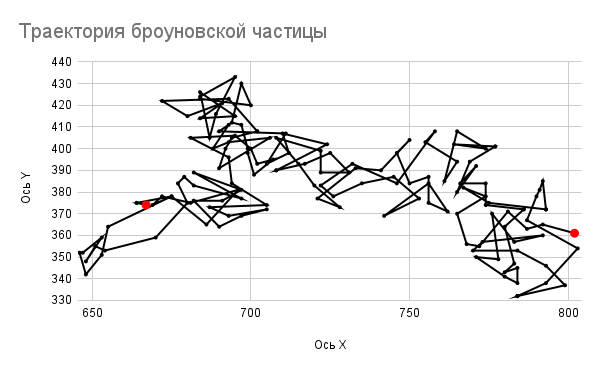
\includegraphics[scale=0.6]{trajectory.png}
    \caption{Движение броуновской частицы. Красным отмечены начальная и конечная точки.}
\end{figure}

Далее, нужно привести графически зависимость $\overline{x^2}$, $\overline{y^2}$, $\frac{\overline{x^2} + \overline{y^2}}{2}$ от $t=n\tau$.

\begin{figure}[ht!]
    \centering
    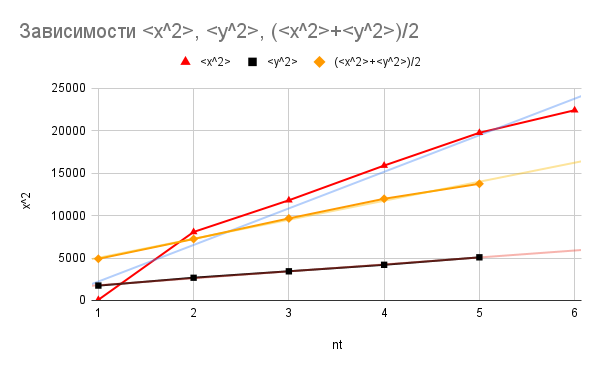
\includegraphics[scale=0.6]{graph.png}
    \caption{Зависимость $\overline{x^2}$, $\overline{y^2}$, $\frac{\overline{x^2} + \overline{y^2}}{2}$ от $t=n\tau$.}
\end{figure}

\clearpage

Далее, нужно перевести пиксели в микрометры.

\begin{table}[!ht]
    \centering
    \begin{tabular}{|l|l|l|}
    \hline
        $x$ & $y$ & $\Delta x$ \\ \hline
        24  & 148 &  \\ \hline
        121 & 148 & 97 \\ \hline
        216 & 152 & 95 \\ \hline
        321 & 154 & 105 \\ \hline
        415 & 156 & 94 \\ \hline
        516 & 156 & 101 \\ \hline
        616 & 156 & 100 \\ \hline
        713 & 159 & 97 \\ \hline
        815 & 159 & 102 \\ \hline
    \end{tabular}
\end{table}

Из таблицы получаем, что $\overline{\Delta x} \approx 98,88 мкм$. С учётом того, что измерение происходит при помощи мышки на экране (что очень неточно), я сделаю грубое предположение, что 100 пикселей = 10 мкм. То есть 10 пикселей = 1 мкм. Далее я буду использовать именно такой коэффициент перевода в мкм, обозначим его за $\aleph$.

Диаметр частицы получился около $d\approx1,8$мкм.
Коэффициент диффузии получился $D\approx171\frac{мкм^2}{с}$

\section{Вывод}

В данной работе были определены коэффициент перевода изображения в микрометры, диаметр частицы и, соответственно, коэффициент диффузии.

$$
\aleph = 1/10
$$
$$
d = 1.8 мкм
$$
$$
D = 171 \frac{мкм^2}{c}
$$

Однако значения $x^2$, $y^2$, $D$ кажутся слишком большими, однако анализ фотографий даёт понять, что частица двигалась очень свободно, на большие  расстояния. Потому при больших t значения оказывались соответственно больше.

\end{document}
